%%%%%%%%%%%%%%%%%%%%%%%%%%%%%%%%%%%%%%%%%%%%%%%%%%%%%%%%%%%%%%%%%%%%%%%%%%%%
%% Author template for INFORMS Journal on Computing (ijoc)
%% Mirko Janc, Ph.D., INFORMS, mirko.janc@informs.org
%% ver. 0.95, December 2010
%%%%%%%%%%%%%%%%%%%%%%%%%%%%%%%%%%%%%%%%%%%%%%%%%%%%%%%%%%%%%%%%%%%%%%%%%%%%
%\documentclass[ijoc,blindrev]{informs3}
\documentclass[11pt]{article} % current default for manuscript submission

\usepackage{fullpage}

% Natbib setup for author-year style
\usepackage{natbib}
  \bibpunct[, ]{(}{)}{,}{a}{}{,}%
  \def\bibfont{\small}%
  \def\bibsep{\smallskipamount}%
  \def\bibhang{24pt}%
  \def\newblock{\ }%
  \def\BIBand{and}%

\usepackage{amsmath,amssymb} 
\def\real{\mathbb{R}}
\def\R{\real}
\def\N{\mathbb{N}}
\def\Z{\mathbb{Z}}
\def\lexmin{\text{lexmin}}
\def\argmin{\text{argmin}}

\usepackage{algorithm}
\usepackage{algcompatible}
\usepackage{float}
\usepackage{graphicx}
\usepackage{xcolor}
%\usepackage{pst-all}
%\usepackage{auto-pst-pdf}
\usepackage{subcaption}

\usepackage{pdflscape}
\usepackage{tabularx}
\usepackage{colortbl}
\usepackage{multirow}
\usepackage{tikz}

\newcommand{\MS}[1]{\begin{color}{red}{#1}\end{color}}
\newcommand{\NB}[1]{\begin{color}{purple}{#1}\end{color}}

\makeatletter
\def\BState{\State\hskip-\ALG@thistlm}
\makeatother
\renewcommand{\algorithmicrequire}{\textbf{Input:}}
\renewcommand{\algorithmicensure}{\textbf{Output:}}

\usepackage[normalem]{ulem}

%%%%%%%%%%%%%%%%
\begin{document}
%%%%%%%%%%%%%%%%

\title{Generating Biobjective Mixed Integer Programming Instances}

\date{}
\maketitle
 
\noindent We provide a method for generating BOMIPs for which the nondominated frontier is known. We present two classes of instances. The first class of instances are BOMIPs whose frontiers are characterized by a set of randomly generated, isolated NDPs. The second class of instances are characterized by a set of deterministically generated NDPs, each the apex of a cone of randomized width. Both classes have complex, intersecting frontiers.

Both classes of instances have the same fundamental structure. Each objective function is equal to one of the two continuous decision variables, i.e. $z_1(x):=x_1$ and $z_2(x):=x_2$, where $x\in\R^2$. Furthermore, a line segment $L$ in the criterion space will have some nondominated portions. Specifically, $L = \{(x_1,x_2)\in\R^2: x_1+x_2=0, -k\leq x_i\leq k\ \text{for}\ i=1,2\}$ where $k\in (0,\infty)$ is a parameter. Portions of the line segment will be dominated by a set of generated NDPs. If $n$ NDPs are generated, then the BOMIP instance will have $n+1$ binary variables, i.e., $y\in\{0,1\}^{n+1}$. Therefore, the feasible set of the BOMIP instance is $\mathbb{X} \subseteq \R^2 \times \{0,1\}^{n+1}$.

Next, we discuss how to generate a set of $n$ NDPs, $\{(a_i,b_i)\}_{i=1,2,...,n}$, where each dominates a portion of $L$. We note two properties that these NDPs must satisfy: (1) if $(a_i,b_i)$ dominates any portion of $L$, then we must have $a_i+b_i<0$ where $a_i,b_i\in[-k,k]$ for all $i$, and (2) if $(a_i,b_i)$ and $(a_j,b_j)$ are two distinct NDPs, then $a_i < a_j$ if and only if $b_i > b_j$. We use $U(x,y)$ to indicate a uniformly distributed random variable bounded within $(x,y)$.

\section{Fixed Cone-Width Instances}\label{Subsec:FixedDistInstances}

While the first class of instances does incorporate some randomness, their frontier is completely known. This is achieved by choosing the $n$ NDPs in such a way that they are each equidistant from $L$ and that two neighboring NDPs do not dominate the same portion of $L$. The former is easily accomplished by defining a line segment parallel to $L$ but shifted vertically down by $d\in(0,\tfrac{2k}{n})$ units as $L_d = \{ (x_1,x_2): x_1 + x_2=-d, -k\leq x_i\leq k-d\ \text{for}\ i=1,2\}$. Then any point on $L_d$ dominates a segment of $L$ and has the same distance to $L$, so we can simply choose $n$ points of $L_d$. 

In order to ensure that any portion of $L$ is not dominated simultaneously by two neighboring NDPs (see Figure~\ref{Fig:FixedDistInstances}), we must choose the NDPs such that $-b_i < a_{i+1}$ for $i=1,2,...,n-1$. This result comes from considering the points $(a_i,b_i)$ and $(a_{i+1},b_{i+1})$ projected onto the line $L$ horizontally and vertically, respectively. By avoiding such overlapping, choosing $(a_1,b_1)$ such that it does not dominate the left endpoint of $L$, and similarly choosing $(a_n,b_n)$ such that it does not dominate the right endpoint of $L$, this procedure will guarantee exactly $n+1$ nondominated segments of $L$. 

\begin{figure}[t!]
\scriptsize
\begin{center}
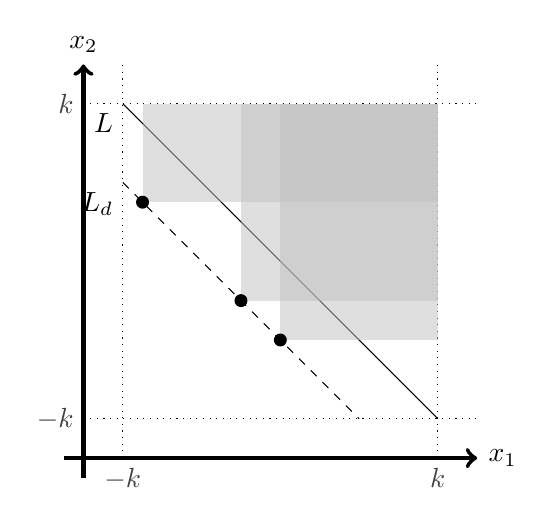
\begin{tikzpicture}[scale=0.5]
%\draw [fill=gray!30,gray!25] (0,0) rectangle (10,10);
%\draw [fill=white,white] (0,0) rectangle (9,5);
\draw[->,ultra thick] (-0.5,0)--(10,0) node[right]{$x_1$};
\draw[->,ultra thick] (0,-0.5)--(0,10) node[above]{$x_2$};

\draw [black, dotted] (0,9) -- (10,9) ;
\node [left,darkgray] at (0,9) {$k$} ;
\draw [black, dotted] (0,1) -- (10,1) ;
\node [left,darkgray] at (0,1) {$-k$} ;

\draw [black, dotted] (9,0) -- (9,10) ;
\node [below, darkgray] at (9,0) {$k$} ;
\draw [black, dotted] (1,0) -- (1,10) ;
\node [below, darkgray] at (1,0) {$-k$} ;

\draw [black] (1,9) -- (9,1);
\node [below left] at (1,9) {$L$};
\draw [black, dashed] (1,7) -- (7,1);
\node [below left] at (1,7) {$L_d$};


\fill[fill=lightgray, fill opacity=0.5] (1.5,9) -- (1.5,6.5) -- (9,6.5) -- (9,9);
\draw [fill] (1.5,6.5) circle [radius=0.15];

\fill[fill=lightgray, fill opacity=0.5] (4,9) -- (4,4) -- (9,4) -- (9,9);
\draw [fill] (4,4) circle [radius=0.15];

\fill[fill=lightgray, fill opacity=0.5] (5,9) -- (5,3) -- (9,3) -- (9,9);
\draw [fill] (5,3) circle [radius=0.15];

\end{tikzpicture} \hspace{1.5cm}
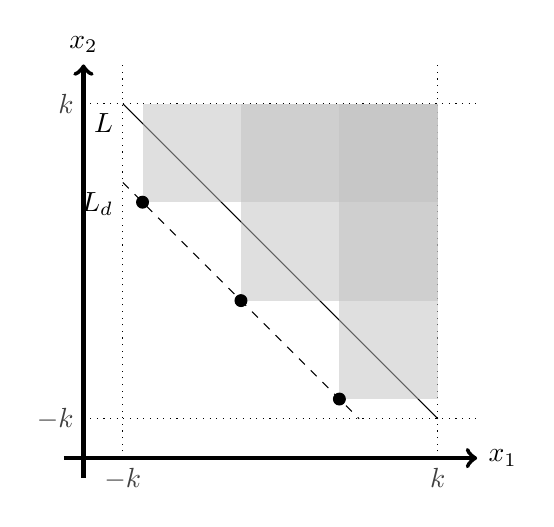
\begin{tikzpicture}[scale=0.5]
\draw[->,ultra thick] (-0.5,0)--(10,0) node[right]{$x_1$};
\draw[->,ultra thick] (0,-0.5)--(0,10) node[above]{$x_2$};

\draw [black, dotted] (0,9) -- (10,9) ;
\node [left,darkgray] at (0,9) {$k$} ;
\draw [black, dotted] (0,1) -- (10,1) ;
\node [left,darkgray] at (0,1) {$-k$} ;

\draw [black, dotted] (9,0) -- (9,10) ;
\node [below, darkgray] at (9,0) {$k$} ;
\draw [black, dotted] (1,0) -- (1,10) ;
\node [below, darkgray] at (1,0) {$-k$} ;

\draw [black] (1,9) -- (9,1);
\node [below left] at (1,9) {$L$};
\draw [black, dashed] (1,7) -- (7,1);
\node [below left] at (1,7) {$L_d$};


\fill[fill=lightgray, fill opacity=0.5] (1.5,9) -- (1.5,6.5) -- (9,6.5) -- (9,9);
\draw [fill] (1.5,6.5) circle [radius=0.15];

\fill[fill=lightgray, fill opacity=0.5] (4,9) -- (4,4) -- (9,4) -- (9,9);
\draw [fill] (4,4) circle [radius=0.15];

\fill[fill=lightgray, fill opacity=0.5] (6.5,9) -- (6.5,1.5) -- (9,1.5) -- (9,9);
\draw [fill] (6.5,1.5) circle [radius=0.15];

\end{tikzpicture}
\caption{NDPs and associated cones generated by the fixed cone-width class of instances. (Left) If the pointed cones from NDPs overlap on $L$, then there are fewer than $n+1$ nondominated segments of $L$. (Right) Choosing the NDPs such that $-b_i < a_{i+1}$ prevents such overlapping, thus guaranteeing exactly $n+1$ line segments of $L$ are nondominated.\label{Fig:FixedDistInstances} }
\end{center}
\end{figure}

To prevent numerical issues, we use $n$ equal-sized subintervals within $(-k,k)$ when choosing the NDPs to prevent dense clustering of the points in any one region. We also guarantee that the nondominated portions of $L$ are no shorter in length than $\epsilon$ by requiring $a_{i+1} > -b_i+\epsilon$. The resulting procedure is given in Algorithm~\ref{Alg:FixedDist}.

\begin{algorithm}[H]
	\caption{Fixed Cone-Width NDP Generation}\label{Alg:FixedDist}
	\small
	\begin{algorithmic}[1]
		\STATE $d=k/4$ (distance by which $L_d$ is shifted down)
		\STATE $w=(2k-d)/n$ (the width of subintervals)
		\STATE $a_1 = U(-k,-k+w)$
		\STATE $b_1 = -a_1 - d$
		\FOR{$i=2,3,...,n$}
		\STATE $a_i = U(\max\{-k+(i-1)w,-b_{i-1}+\epsilon\},-k+iw)$ 
		\STATE $b_i = -a_i - d$
		\ENDFOR
	\end{algorithmic}
\end{algorithm}

For constructing the associated BOMIP, assume that the line $L$, NDPs $\{(a_i,b_i)\}_{i=1..n}$, and parameters $k$, $n$ are known. With $\vec{z}((x,y))=(x_1,x_2)$ as our objective vector, we set the uniform bound $-k\leq x_i \leq k$ for $i=1,2$. Then we have the following polytopes of interest in the criterion space: 
\begin{itemize}
\item The line segment $L$ is the nondominated frontier of the polytope 
$$P_0 = \{(x_1,x_2): x_1+x_2\geq 0, -k\leq x_i \leq k, i=1,2\}.$$
\item For $i=1,2,...,n$, the \textit{orthogonal} pointed cone\footnote{The fact that we use the orthogonal pointed cone (with radius of 90 degrees) for \textit{all} NDPs led to the name of ``fixed cone-width.''} dominated by its vertex NDP $(a_i,b_i)$ is defined by
$$P_i =\{(x_1,x_2):\ x_1 \geq a_i,\ x_2 \geq b_i \}.
$$
\end{itemize}
To have the exact nondominated frontier we desire, we require any NDP $(x^*_1,x^*_2)$ to belong to at least one of these polytopes (since the polytopes intersect, it may belong to more than one). Let $y\in\{0,1\}^{n+1}$ be a binary decision vector, where $y_0=1$ implies $(x^*_1,x^*_2)\in L$ and for $i=1,2,...,n$, $y_i=1$ indicates that $(x^*_1,x^*_2)\in P_i$ for $i=0,1,...,n$. We also require $\sum_{i=0}^n y_i =1$. We therefore define an MILP with constraints that enforce such implications (note we do not enforce that $y_i=0$ implies $(x^*_1,x^*_2)\not\in P_i$). The associated MILP for the first class of instances is thus defined as:
\begin{align}
\text{minimize}\hspace{1.7cm} (x_1,x_2) \nonumber \\
\text{s.t.}\hspace{1.7cm} x_1+x_2 &\geq -2k(1-y_0) \label{MILP:Lconstraint} \\
x_1 &\geq a_i -2k(1-y_i) \hspace{0.5cm} \forall i=1,2,...,n \label{MILP:Aconstraint} \\
x_2 &\geq b_i -2k(1-y_i) \hspace{0.5cm} \forall i=1,2,...,n \label{MILP:Bconstraint} \\
\sum_{i=0}^{n} y_i &=1 \\ 
-k \leq x_i &\leq k \hspace{1.5cm} \forall i=1,2 \label{MILP:bounds} \\
y&\in\{0,1\}^{n+1}. \nonumber 
\end{align}

Observe that when $y_0=1$, we have that \eqref{MILP:Lconstraint} and \eqref{MILP:bounds} together characterize the polytope $P_0$ containing the line segment $L$. Similarly, when $y_i=1$ for $i=1,...,n$, \eqref{MILP:Aconstraint} and \eqref{MILP:Bconstraint} together characterize the pointed cone polytope $P_i$ containing NDP $(a_i,b_i)$. Otherwise, when $y_i=0$ for $i=0,1,...,n$, the associated constraints from \eqref{MILP:Lconstraint}, \eqref{MILP:Aconstraint}, and \eqref{MILP:Bconstraint} including $y_i$ become redundant.

By construction, we are guaranteed to have $n+1$ distinct binary vectors ($e_1,e_2,...,e_{n+1}$) that each belong to at least one efficient solution in the efficient frontier. The nondominated frontier associated with this BOMIP has exactly $n$ isolated NDPs and $n+1$ line segments (2 half-open at the ends of $L$ and $n-1$ open segments in between isolated NDPs). 

\textit{Note: Even large instances of this class of BOMIPs are solved quite quickly by most methods, so they are not ideal for testing computational efficiency. However, since the nondominated frontiers are known exactly, they can be used for \textit{validating} the correctness of an algorithm.}

\section{Randomized Cone-Width Instances}\label{Subsec:RandDistInstances}

The second class of instances randomizes the pointed cones associated with each NDP rather than only using orthogonal pointed cones. Similar to the first class of instances, we restrict the cones of the NDPs from overlapping the same portion of $L$, as in Figure~\ref{Fig:RandDistInstances}, which requires a careful choice of the NDPs. We postpone a discussion of how to choose the NDPs until after introducing the randomizing of cone widths.

\begin{figure}[t!]
\scriptsize
\begin{center}
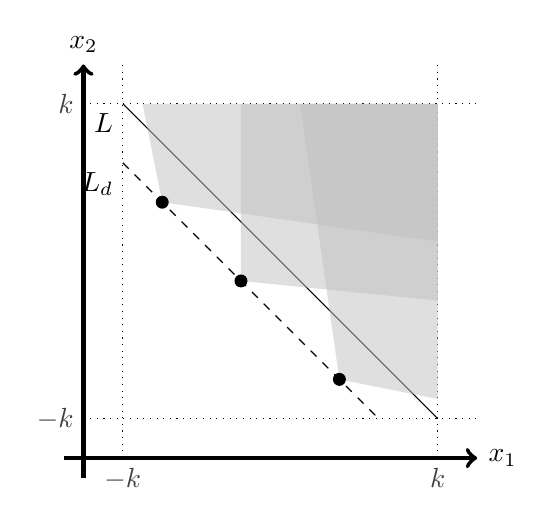
\begin{tikzpicture}[scale=0.5]
\draw[->,ultra thick] (-0.5,0)--(10,0) node[right]{$x_1$};
\draw[->,ultra thick] (0,-0.5)--(0,10) node[above]{$x_2$};

\draw [black, dotted] (0,9) -- (10,9) ;
\node [left,darkgray] at (0,9) {$k$} ;
\draw [black, dotted] (0,1) -- (10,1) ;
\node [left,darkgray] at (0,1) {$-k$} ;

\draw [black, dotted] (9,0) -- (9,10) ;
\node [below, darkgray] at (9,0) {$k$} ;
\draw [black, dotted] (1,0) -- (1,10) ;
\node [below, darkgray] at (1,0) {$-k$} ;

\draw [black] (1,9) -- (9,1);
\node [below left] at (1,9) {$L$};
\draw [black, dashed] (1,7.5) -- (7.5,1);
\node [below left] at (1,7.5) {$L_d$};


\fill[fill=lightgray, fill opacity=0.5] (1.5,9) -- (2,6.5) -- (9,5.5) -- (9,9);
\draw [fill] (2,6.5) circle [radius=0.15];

\fill[fill=lightgray, fill opacity=0.5] (4,9) -- (4,4.5) -- (9,4) -- (9,9);
\draw [fill] (4,4.5) circle [radius=0.15];

\fill[fill=lightgray, fill opacity=0.5] (5.5,9) -- (6.5,2) -- (9,1.5) -- (9,9);
\draw [fill] (6.5,2) circle [radius=0.15];

\end{tikzpicture}
\vspace{0.2cm}
\caption{NDPs and associated cones generated by the randomized cone-width class of instances. \label{Fig:RandDistInstances} }
\end{center}
\end{figure}

Let $(a,b)$ be a point that dominates line $L$. Note that the simple orthogonal pointed cone with $(a,b)$ as its vertex is given by $\{(x_1,x_2)\in\R^2: x_1 \geq a, x_2 \geq b\}$, as before. We will generalize these inequalities, as shown in Figure~\ref{Fig:PointedCone}. To define any pointed cone with the vertex $(a,b)$, requires two inequalities of the form 
\begin{align}
\theta_1 x_1 + (1-\theta_1)x_2 \geq \theta_1 a + (1-\theta_1)b \label{Eq:Cone1} \\
\theta_2 x_1 + (1-\theta_2)x_2 \geq \theta_2 a + (1-\theta_2)b. \label{Eq:Cone2}
\end{align}
The cones must be derived from $\theta_1 \in [0,\frac{1}{2})$ and $\theta_2 \in (\frac{1}{2},1]$ based on the following observations. First, a line defined by the inequalities held at strict equality -- that is neither horizontal ($\theta_i = 0$) nor vertical ($\theta_i=1$) -- must both have negative slope, i.e. $-\frac{\theta_i}{1-\theta_i}<0$, so $\theta_i$ must be within $(0,1)$. Second, neither line may be parallel to $L$, so $-\frac{\theta_i}{1-\theta_i}\neq -1$ and so $\theta_i \neq \frac{1}{2}$. Lastly, in order for both edges of the pointed cone to contribute to the nondominated frontier, we require $\theta_1 <\frac{1}{2}$ and $\theta_2 >\frac{1}{2}$. 


\begin{figure}[t!]
\scriptsize
\begin{center}
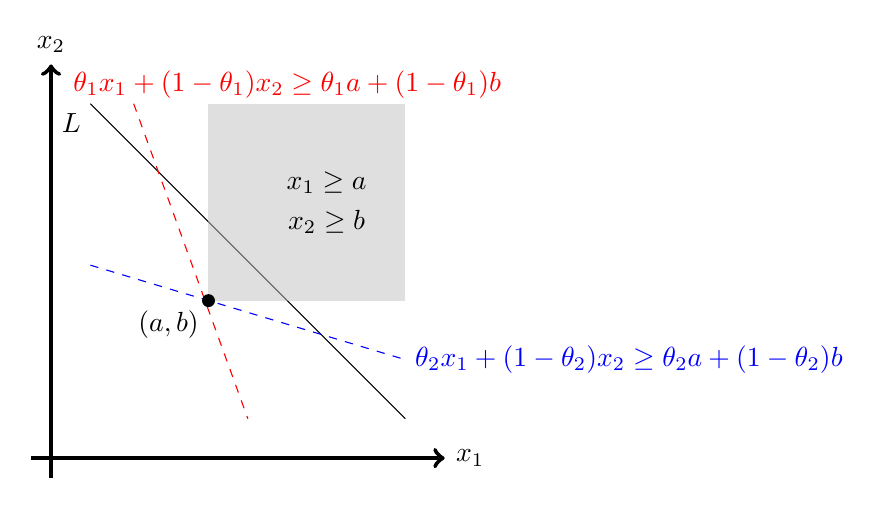
\begin{tikzpicture}[scale=0.5]
\draw[->,ultra thick] (-0.5,0)--(10,0) node[right]{$x_1$};
\draw[->,ultra thick] (0,-0.5)--(0,10) node[above]{$x_2$};

\draw [black] (1,9) -- (9,1);
\node [below left] at (1,9) {$L$};

\fill[fill=lightgray, fill opacity=0.5] (4,9) -- (4,4) -- (9,4) -- (9,9);
\node at (7,7) {$x_1\geq a$};
\node at (7,6) {$x_2\geq b$};
\draw [dashed,blue] (1,4.9) -- (9,2.5);
\node [right, blue] at (9,2.5) {$\theta_2 x_1 + (1-\theta_2)x_2 \geq \theta_2 a + (1-\theta_2)b$};
\draw [dashed,red] (2.1,9) -- (5,1);
\node [red] at (6,9.5) {$\theta_1 x_1 + (1-\theta_1)x_2 \geq \theta_1 a + (1-\theta_1)b$};
\draw [fill] (4,4) circle [radius=0.15];
\node [below left] at (4,4) {$(a,b)$};

\end{tikzpicture} 
\caption{The orthogonal pointed cone with vertex $(a,b)$ is shaded. The generalized pointed cone is defined between the red and blue inequalities. We randomize the cone widths by choosing $\theta_1$ and $\theta_2$.\label{Fig:PointedCone}}
\end{center}
\end{figure}

The orthogonal cone given by $x_1 \geq a$ and $x_2 \geq b$ results from substituting $\theta_1=1$ and $\theta_2=0$ into \eqref{Eq:Cone1} and\eqref{Eq:Cone2}, respectively. Having some orthogonal cones is desired in order to induce some isolated points (and open endpoints) into the nondominated frontier. Therefore, we define a parameter $\pi\in[0,1]$ representing the probability that a cone is orthogonal. In practice, we use $\pi=0.05$. Algorithm~\ref{Alg:RandTheta} shows how we generate a list of ordered pairs of thetas. 

\begin{algorithm}[H]
	\caption{Theta Generation}\label{Alg:RandTheta}
	\small
	\begin{algorithmic}[1]
		\STATE thetalist$=\emptyset$
		\FOR{$i=1,2,...,n$}
		\IF{$U(0,1)\leq \pi$}
		\STATE $\theta_1 = 0$
		\STATE $\theta_2 = 1$
		\ELSE
		\STATE $\theta_1 = U(0,\frac{1}{4})$
		\STATE $\theta_2 = U(\frac{3}{4},1)$
		\ENDIF 
		\STATE thetalist.append$\left( (\theta_1,\theta_2) \right)$
		\ENDFOR
	\end{algorithmic}
\end{algorithm}

We tighten the bounds on $\theta_1, \theta_2$ to yield smaller-width pointed cones, namely $\theta_1\in[0,\frac{1}{4})$ and $\theta_2\in(\frac{3}{4},1]$. 
Note that these bounds on the slopes of the linear inequalities allow us to compute the minimum distance between two NDPs required to ensure that their cones do not overlap on the line segment $L$. By a geometric argument, we have that if all NDPs are chosen from a line segment shifted down $d$ from $L$, i.e. $L_d$, then any two neighboring NDPs should be at least distance $2d$ from each other in both coordinates. To ensure that the nondominated portions of $L$ have length of at least $\epsilon$, we force NDPs to be at least $2d+1$ apart. If we have $n+1$ of such intervals (one for each NDP and one additional to allow for the endpoints of $L$ to be nondominated), then we can compute the appropriate $d$ in order to fit $n$ NDPs within our bounds, $x_i\in [-k,k]$ for $i=1,2$:
$$ (n+1)(2d+1) = 2k \quad \Leftrightarrow \quad  d = \tfrac{k}{n+1} - \tfrac{1}{2}. $$
This results in Algorithm~\ref{Alg:RandNDPs} for generating the NDPs for this class of instances.

\begin{algorithm}[H]
	\caption{Randomized Cone-Width NDP Generation}\label{Alg:RandNDPs}
	\small
	\begin{algorithmic}[1]
		\STATE $d=k/(n+1)-0.5$
		\STATE $a_1 = -k + 0.5 d$
		\STATE $b_1 = -a_1-d$
		\FOR{$i=2,...,n$}
		\STATE $a_i = a_{i-1}+2d+1$ 
		\STATE $b_i = -a_i-d$
		\ENDFOR
	\end{algorithmic}
\end{algorithm}

The BOMILP for the second class of instances is defined as:
\begin{align}
\text{minimize}\hspace{1.7cm} (x_1,x_2) \nonumber \\
\text{s.t.}\hspace{1.7cm} x_1+x_2 &\geq -2k(1-y_0) \label{Eq:LineConstraint}\\ 
\theta^i_1 x_1 + (1-\theta^i_1)x_2 &\geq \theta^i_1 a_i + (1-\theta^i_1)b_i -2k(1-y_i) \hspace{0.5cm} \forall i=1,2,...,n \label{Eq:ThetaConstraint1} \\ 
\theta^i_2 x_1 + (1-\theta^i_2)x_2 &\geq \theta^i_2 a_i + (1-\theta^i_2)b_i -2k(1-y_i) \hspace{0.5cm} \forall i=1,2,...,n \label{Eq:ThetaConstraint2} \\
\sum_{i=0}^n y_i &=1 \\
-k \leq x_i &\leq k \hspace{1.5cm} \forall i=1,2 \\
z&\in\{0,1\}^{n+1} \nonumber
\end{align}
By construction, we will have no more than $n+1$ distinct binary vectors that each belong to at least one efficient solution in the efficient frontier. The nondominated frontiers associated with this BOMIP will have no more than $3n+1$ line segments ($n+1$ from $L$ and at most 2 per NDP), including open endpoints induced by any orthogonal cones and closed endpoints induced by intersecting slices. 

Note that the BOMIP for both classes of instances has $n+3$ variables and $4+2n$ constraints, so the size of the problem is linear with respect to $n$. 

\textit{Note: The second class of instances, compared to the first class, is more difficult to solve because of the high frequency of intersecting integer slices in the frontier.}

\section{Bent Randomized Cone-Width Instances}
\label{Subsec:BentInstances}

As the name suggests, the bent randomized cone-width instances represent a variation of the randomized cone-width instance. It employs the same method for generating the $n$ NDPs (at uniform distance from $L$) and their cone widths. However, the straight line segment $L$ is replaced by a slightly bent line segment, $\hat{L}$, i.e. the boundary of a cone that is very wide (see Figure~\ref{Fig:BentInstance}). 

\begin{figure}[t!]
	\scriptsize
	\begin{center}
		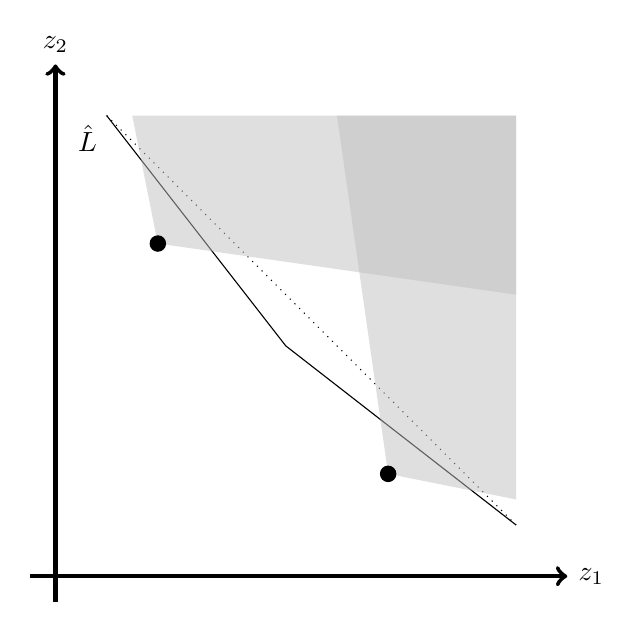
\begin{tikzpicture}[scale=0.65]
		\draw[->,ultra thick] (-0.5,0)--(10,0) node[right]{$z_1$};
		\draw[->,ultra thick] (0,-0.5)--(0,10) node[above]{$z_2$};
		
		\draw [black, dotted] (1,9) -- (9,1);
		\draw [black] (1,9) -- ( 4.5,4.5) -- (9,1);
		\node [below left] at (1,9) {$\hat{L}$};
		%\draw [black, dashed] (1,7.5) -- (7.5,1);
		
		\fill[fill=lightgray, fill opacity=0.5] (1.5,9) -- (2,6.5) -- (9,5.5) -- (9,9);
		\draw [fill] (2,6.5) circle [radius=0.15];
		
		\fill[fill=lightgray, fill opacity=0.5] (5.5,9) -- (6.5,2) -- (9,1.5) -- (9,9);
		\draw [fill] (6.5,2) circle [radius=0.15];
		
		\end{tikzpicture}
		\caption{A Bent Randomized Cone-Width instance for $n=2$. The bent line segment $\hat{L}$ comprises two line segments of a very wide cone. Solving a scalarized IP with respect to the gradient of either piece has at most one optimal solution but (for large $n$) multiple near-optimal solutions. \label{Fig:BentInstance} }
	\end{center}
\end{figure}
Now, when solving a scalarized IP with respect to the gradient of either part of the bent line segment, there are no longer multiple optimal solutions, but there are many \textit{near}-optimal solutions.

The ``bent'' line segment has corner point $(a_0, b_0)=(-d/4, -d/4)$, which may be dominated or nondominated, $\theta^0_1=(k+d/4)/(2k)$, and $\theta^0_2=(k-d/4)/(2k)$. Then the bent line segment $\hat{L}$ fits the previous definition for a cone while substituting the corner point $(a_0,b_0)$, $\theta^0_1$, and $\theta^0_2$. Therefore, in the BOMIP for the randomized cone-width instances, we replace constraint \eqref{Eq:LineConstraint} with two constraints of the form \eqref{Eq:ThetaConstraint1} and \eqref{Eq:ThetaConstraint2}. Let the generated NDPs be $\{(a_i,b_i)\}_{i=0,1,...,n}$ and their cones be defined by $\{(\theta^i_1,\theta^i_2)\}_{i=0,1,...,n}$. We then have the following BOMIP for the bent randomized cone-width instance:
\begin{align}
\text{minimize}\hspace{1.7cm} (x_1,x_2) \nonumber \\
\text{s.t.}\quad \theta^i_1 x_1 + (1-\theta^i_1)x_2 &\geq \theta^i_1 a_i + (1-\theta^i_1)b_i -2k(1-y_i) \hspace{0.5cm} \forall i=0,1,2,...,n \\
\theta^i_2 x_1 + (1-\theta^i_2)x_2 &\geq \theta^i_2 a_i + (1-\theta^i_2)b_i -2k(1-y_i) \hspace{0.5cm} \forall i=0,1,2,...,n \\
\sum_{i=0}^n y_i &=1 \\
-k \leq x_i &\leq k \hspace{1.5cm} \forall i=1,2 \\
y&\in\{0,1\}^{n+1}. \nonumber
\end{align}


%%%%%%%%%%%%%%%%%
\end{document}
%%%%%%%%%%%%%%%%%





